\documentclass[titlepage, a4paper, 12pt] {article}

\usepackage{lmodern}
\usepackage{ifxetex,ifluatex}
\usepackage{fixltx2e} 
\usepackage{amsmath}
\usepackage{txfonts}
\usepackage{amssymb}
\usepackage{times}
\usepackage{graphicx}
\usepackage{epsfig,tabularx,amssymb,amsmath,subfigure,multirow}
%\usepackage{algorithmic}
\usepackage[linesnumbered,ruled,noend]{algorithm2e}
\usepackage[noend]{algorithmic}
\usepackage{multirow}
\usepackage{graphicx,floatrow}
\usepackage{listings}
\usepackage{threeparttable}
%\usepackage{tikz}
\usepackage[T1]{fontenc}
\usepackage{pgfplots}
\usepackage{filecontents}

%\usepackage{setspace}
%\usepackage{marginnote}
%\usepackage{verbatim}
%\usepackage{paralist}
%\usepackage{indentfirst}
%\usepackage{amsthm}
\usepackage{booktabs}
\usepackage{tabularx}
%\usepackage{warpcol}
%\usepackage{longtable}
%\usepackage{syntonly}
%\usepackage[svgnames] {xcolor}
%\usepackage{xcolor}
%\usepackage{multido}
%\usepackage{pst-node}
%\usepackage{pst-tree}
%\usepackage{pst-plot}
%\usepackage{pst-func}
%\usepackage{listings}
%QUERY:why this can not be used here
%\usepackage{makeidx}
\usepackage[colorlinks]{hyperref}
\usepackage{comment}

\lstset{%
	alsolanguage=Java,
	%language={[ISO]C++},       %language为,还有{[Visual]C++}
	%alsolanguage=[ANSI]C,      %可以添加很多个alsolanguage,如alsolanguage=matlab,alsolanguage=VHDL等
	%alsolanguage= tcl,
	alsolanguage= XML,
	tabsize=4, %
	frame=shadowbox, %把代码用带有阴影的框圈起来
	commentstyle=\color{red!50!green!50!blue!50},%浅灰色的注释
	rulesepcolor=\color{red!20!green!20!blue!20},%代码块边框为淡青色
	keywordstyle=\color{blue!90}\bfseries, %代码关键字的颜色为蓝色,粗体
	showstringspaces=false,%不显示代码字符串中间的空格标记
	stringstyle=\ttfamily, % 代码字符串的特殊格式
	keepspaces=true, %
	breakindent=22pt, %
	numbers=left,%左侧显示行号 往左靠,还可以为right,或none,即不加行号
	stepnumber=1,%若设置为2,则显示行号为1,3,5,即stepnumber为公差,默认stepnumber=1
	%numberstyle=\tiny, %行号字体用小号
	numberstyle={\color[RGB]{0,192,192}\tiny} ,%设置行号的大小,大小有tiny,scriptsize,footnotesize,small,normalsize,large等
	numbersep=8pt,  %设置行号与代码的距离,默认是5pt
	basicstyle=\footnotesize, % 这句设置代码的大小
	showspaces=false, %
	flexiblecolumns=true, %
	breaklines=true, %对过长的代码自动换行
	breakautoindent=true,%
	breakindent=4em, %
	%	escapebegin=\begin{CJK*}{GBK}{hei},escapeend=\end{CJK*},
	aboveskip=1em, %代码块边框
	tabsize=2,
	showstringspaces=false, %不显示字符串中的空格
	backgroundcolor=\color[RGB]{245,245,244},   %代码背景色
	%backgroundcolor=\color[rgb]{0.91,0.91,0.91}    %添加背景色
	escapeinside=``,  %在``里显示中文
	%% added by http://bbs.ctex.org/viewthread.php?tid=53451
	fontadjust,
	captionpos=t,
	framextopmargin=2pt,framexbottommargin=2pt,abovecaptionskip=-3pt,belowcaptionskip=3pt,
	xleftmargin=4em,xrightmargin=4em, % 设定listing左右的空白
	texcl=true,
	% 设定中文冲突,断行,列模式,数学环境输入,listing数字的样式
	extendedchars=false,columns=flexible,mathescape=true
	% numbersep=-1em
}

\setlength{\parindent} {0pt}
\addtolength{\parskip} {3pt}
\linespread{1.3}

%QUERY+BETTER:how to remove box for links

\begin{document}

\title{\textbf{Test Report on gStore}}
\author{Li Zeng\footnote{EECS of Peking University, zengli-bookug@pku.edu.cn}}
\date{\today}
\maketitle

\setcounter{tocdepth}{3}
\tableofcontents
\clearpage

\section{Preface}

gStore\footnote{\href{https://github.com/Caesar11/gStore}{https://github.com/Caesar11/gStore}} is a graph-based database management system, which keeps the structure of original RDF\footnote{\href{http://www.w3school.com.cn/rdf/}{http://www.w3school.com.cn/rdf/}} data. 

The data model is directed graph with labels, and each vertex corresponds to a subject or object. 

Given a SPARQL\footnote{\href{https://www.w3.org/TR/sparql11-query/}{https://www.w3.org/TR/sparql11-query/}} query(only select...where clause is well supported now), gStore will transfer it to a directed graph with labels first.

Then the query problem will be equivalent to a subgraph matching problem.
An index called VSTree is used in gStore to speed up the matching process. For each variable in the SPARQL query, gStore acquires its candidates through VSTree, and finally a join process is performed to get the final result.  \\

We compare the performance of gStore with apache-jena\footnote{\href{http://jena.apache.org/}{http://jena.apache.org/}}, openrdf-sesame\footnote{\href{http://www.rdf4j.org/}{http://www.rdf4j.org/}} and virtuoso-openlinksw\footnote{\href{http://virtuoso.openlinksw.com/}{http://virtuoso.openlinksw.com/}} on several RDF datasets.
The items needing to be considered include the time to build database, the size of database and the time to answer each SPARQL query.
In addition, we will give a special explanation if the query results of each database do not match.
(we will not consider the memory and disk cost except for special cases) \\

\clearpage

\section{Environment Setup}

We need to do some preparations before the experiment to ensure all datasets and corresponding queries 
can be run correctly by all database management systems. The limitations are listed below:

\begin{enumerate}
	\item gStore does not support queries with unbounded predicates
	\item Jena does not support datasets with prefix declarations
	\item Sesame does not support entities without appropiate prefixes
	\item Virtuoso will remove the '<' and '>' for entities, '"' for literals 
\end{enumerate} 

We should not include the time to load database indexes(called offline time) when comparing the time to answer SPARQL queries. And we need to empty the buffer and cache of operation system when the experiment for each database management system is over. 

The datasets used include WatDiv\footnote{\href{http://dsg.uwaterloo.ca/watdiv/}{http://dsg.uwaterloo.ca/watdiv/}}, 
LUBM\footnote{\href{http://swat.cse.lehigh.edu/projects/lubm/}{http://swat.cse.lehigh.edu/projects/lubm/}}, BSBM\footnote{\href{https://sourceforge.net/projects/bsbmtools/files/bsbmtools/}{https://sourceforge.net/projects/bsbmtools/files/bsbmtools/}} and DBpedia\footnote{\href{http://wiki.dbpedia.org/}{http://wiki.dbpedia.org/}}. DBpedia are the background data of wikipedia, 
while the others are generated by programs. SPARQL queries are generated by programs or written manually. 

When testing BSBM and DBpedia, some queries contain "\^{}\^{}" and gStore will ouput nothing in these cases.
In addition, if the output results contain "\^{}\^{}", gStore and Virtuoso will ignore the properties linked by "\^{}\^{}".
What is more, Sesame does not support LUBM due to invalid IRI, and it is unable to deal with too large datasets like dbpedia2014, watdiv\_300M, bsbm\_100000. Virtuoso can not deal with watdiv\_300M, lubm\_5000 and dbpedia2014, neither. 

\clearpage

The experiment is finished on a Linux server with 82G memory and 7T disk. CentOS2.6.32-573.3.1.el6.x86\_64 is 
installed and we require that the version of glibc should be at least 2.14. 

The versions of all database management systems used here are all open source. Latest versions are choosed, 
i.e. 3.0.1 for apache-jena, 4.1.1 for openrdf-sesame and 7.2 for virtuoso-openlinksw.

\clearpage

\section{Experiment Result}

All results are saved in load.log/, result.log/ and time.log/, and the format is TSV. 

Table \ref{table:loading} shows the index size and loading time of the datasets
for different systems.

\begin{table}[htcp]
	\small
	\begin{threeparttable}
		\begin{tabular}{|c||c|c|c||c|c|c|}
			\hline
			& \multicolumn{3}{c||}{Index Size(KB)}& \multicolumn{3}{c|}{Loading Time(ms)}\\
			\hline
			\hline
			Datasets & gStore & Jena& Virtuoso& gStore & Jena& Virtuoso\\
			\hline
			DBpedia 2014 & 42,415,852&	23,151,272 &	-\tnote{$1$} & 8,639,666	&15,555,000	& -	\\
			\hline
			Bsbm 10000 & 1,814,480 & 718,024 & 2,080,000 & 244,153 & 76,000 & 59999  \\
			\hline
			Bsbm 100000 & 12,369,232 & 7,007,988 & 4,390,000 & 2,259,036 & 681,000 & 507,647 \\
			\hline
			LUBM 500  &2,171,084 &1,022,528	&	38,000,000 &	291,382&	94,000 &100,532	 \\
			\hline
			LUBM 5000 & 23,397,548&	10,262,524	 &	- & 3,767,764	&1,098,000  &	- \\
			\hline
			WatDiv 10M & 2,563,168&	1,315,764	 &	10,320,000 & 532,542	&304,000	&225,464 \\
			\hline
			WatDiv 100M & 26,566,780&	13,286,608	 &	8,615,100 & 7,879,602	&20,969,000	&16,981,470 \\
			\hline
			WatDiv 300M & 80,166,500&	38,108,940	 &	- & 19,864,431	&25,041,000 &	- \\
			\hline
		\end{tabular}
		\begin{tablenotes}
			\small
		\item[$1$] ``-'' means that loading does not terminate in 20 hour
		\end{tablenotes}
	\end{threeparttable}
	\caption{Offline Performance}
	\label{table:loading}
\end{table}

The performance of different database management systems is shown in Figures \ref{fig:dbpedia2014Performance}, \ref{fig:Bsbm10000Performance}, \ref{fig:LUBMPerformance} and \ref{fig:WatDivPerformance}.

\begin{figure}[b]%
	\resizebox{0.48\columnwidth}{!}{
			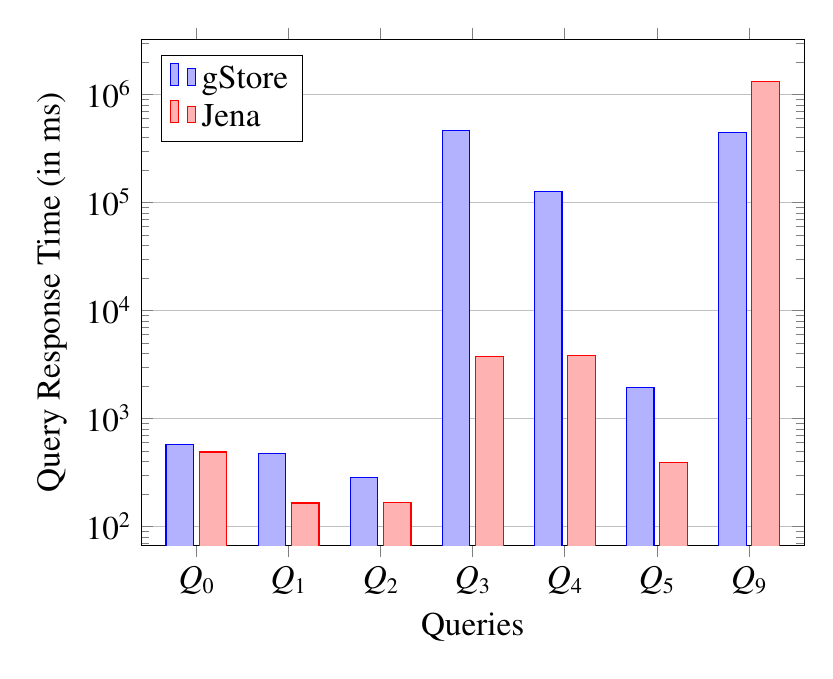
\begin{tikzpicture}[font=\large]
 		 \begin{semilogyaxis}[
               width = 10cm,
               height = 8cm,
    			ybar,
    			%ymin = 1,
    			%ymax = 5000000000,
%    ytick = {1,10,100,1000,10000,100000,1000000,10000000},
   			ymajorgrids = true,
   			ylabel = {Query Response Time (in ms)},
    			xlabel = {Queries},
    			symbolic x coords = {$Q_0$,$Q_1$,$Q_2$,$Q_3$,$Q_4$,$Q_5$,$Q_9$},
    			scaled y ticks = true,
			legend pos= north west,
 legend cell align=left
   		]
   \addplot coordinates {($Q_0$, 578) ($Q_1$, 477) ($Q_2$, 285) ($Q_3$, 465076) ($Q_4$, 127530) ($Q_5$, 1929) ($Q_9$, 447741)};

   \addplot coordinates {($Q_0$, 490) ($Q_1$, 165) ($Q_2$, 166) ($Q_3$, 3727) ($Q_4$, 3847) ($Q_5$, 393) ($Q_9$, 1309775)};

		
   		 \legend{gStore,Jena,Jena}
  		\end{semilogyaxis}
\end{tikzpicture}

	}
	\caption{Query Performance over DBpedia 2014}%
	\label{fig:dbpedia2014Performance}
\end{figure}

\begin{figure}%
	\subfigure[BSBM 10000]{%
		\resizebox{0.8\columnwidth}{!}{
				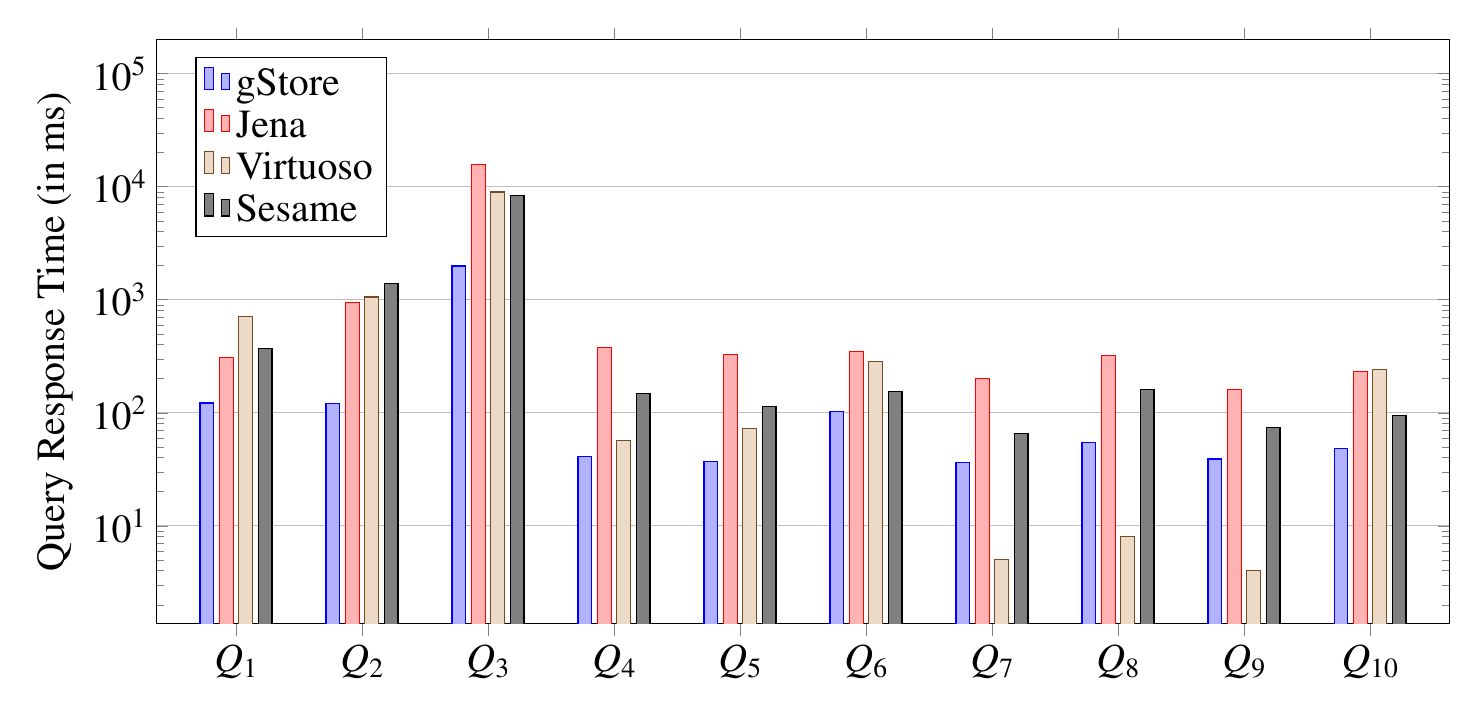
\begin{tikzpicture}[font=\Large]
 		 \begin{semilogyaxis}[
                width = 18cm,
               height = 9cm ,
               ymax=200000,
    			ybar,
   			ymajorgrids = true,
   			ylabel = {Query Response Time (in ms)},
                %xlabel = {Queries},
    			symbolic x coords = {$Q_{1}$,$Q_{2}$,$Q_{3}$,$Q_{4}$,$Q_{5}$,$Q_{6}$,$Q_{7}$,$Q_{8}$,$Q_{9}$,$Q_{10}$},
    bar width=5pt,
             enlarge x limits=0.07,
    			scaled y ticks = true,
			legend pos= north west,
 legend cell align=left
   		]
   \addplot coordinates {($Q_{1}$, 122) ($Q_{2}$, 121) ($Q_{3}$, 1989) ($Q_{4}$, 41) ($Q_{5}$, 37) ($Q_{6}$, 102) ($Q_{7}$, 36) ($Q_{8}$, 55) ($Q_{9}$, 39) ($Q_{10}$, 48) };


\addplot coordinates {($Q_{1}$, 308) ($Q_{2}$, 943) ($Q_{3}$, 15805) ($Q_{4}$, 375) ($Q_{5}$, 327) ($Q_{6}$, 346) ($Q_{7}$, 202) ($Q_{8}$, 322) ($Q_{9}$, 162) ($Q_{10}$, 230)};


\addplot coordinates {($Q_{1}$, 715) ($Q_{2}$, 1059) ($Q_{3}$, 8987) ($Q_{4}$, 57) ($Q_{5}$, 73) ($Q_{6}$, 283) ($Q_{7}$, 5) ($Q_{8}$, 8) ($Q_{9}$, 4) ($Q_{10}$, 242) };

\addplot coordinates {($Q_{1}$, 368) ($Q_{2}$, 1396) ($Q_{3}$, 8312) ($Q_{4}$, 148) ($Q_{5}$, 114) ($Q_{6}$, 154) ($Q_{7}$, 66) ($Q_{8}$, 160) ($Q_{9}$, 74) ($Q_{10}$, 95) };

		
   		 \legend{gStore,Jena,Virtuoso,Sesame}
  		\end{semilogyaxis}
\end{tikzpicture}

		}	
		\label{fig:Bsbm10000Performance}%
	}
	\\
	\subfigure[BSBM 100000]{%
		\resizebox{0.8\columnwidth}{!}{
			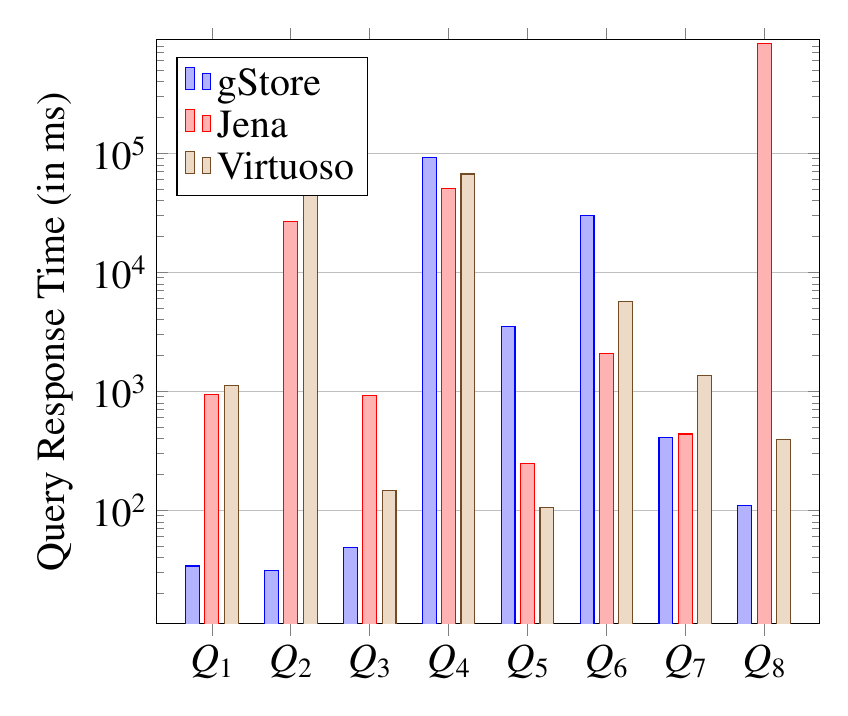
\begin{tikzpicture} [font=\Large]
\begin{semilogyaxis} [
    width = 10cm,
    height = 9cm ,
    ymax=900000,
    ybar,
    ymajorgrids = true,
    ylabel = {Query Response Time (in ms)},
    %xlabel = {Queries},
    symbolic x coords = {$Q_{1}$,$Q_{2}$,$Q_{3}$,$Q_{4}$,$Q_{5}$,$Q_{6}$,$Q_{7}$,$Q_{8}$},
    bar width=5pt,
    enlarge x limits=0.10,
    scaled y ticks = true,
    legend pos= north west,
    legend cell align=left
]
\addplot coordinates {($Q_{1}$, 34) ($Q_{2}$, 31) ($Q_{3}$, 49) ($Q_{4}$, 92688) ($Q_{5}$, 3480) ($Q_{6}$, 30020) ($Q_{7}$, 409) ($Q_{8}$, 109) };

\addplot coordinates {($Q_{1}$, 939) ($Q_{2}$, 26888) ($Q_{3}$, 926) ($Q_{4}$, 50256) ($Q_{5}$, 249) ($Q_{6}$, 2061) ($Q_{7}$, 437) ($Q_{8}$, 837756) };

\addplot coordinates {($Q_{1}$, 1122) ($Q_{2}$, 47059) ($Q_{3}$, 146) ($Q_{4}$, 66916) ($Q_{5}$, 105) ($Q_{6}$, 5654) ($Q_{7}$, 1364) ($Q_{8}$, 392) };

\legend{gStore,Jena,Virtuoso,Sesame}
\end{semilogyaxis}
\end{tikzpicture}

		}
		\label{fig:BSBM100000Performance}%
	}
	\caption{Query Performance over Bsbm}%
	\label{fig:BSBMPerformance}
\end{figure}

%\clearpage

\begin{figure}[t]%
	\subfigure[LUBM 500]{%
		\resizebox{0.98\columnwidth}{!}{
				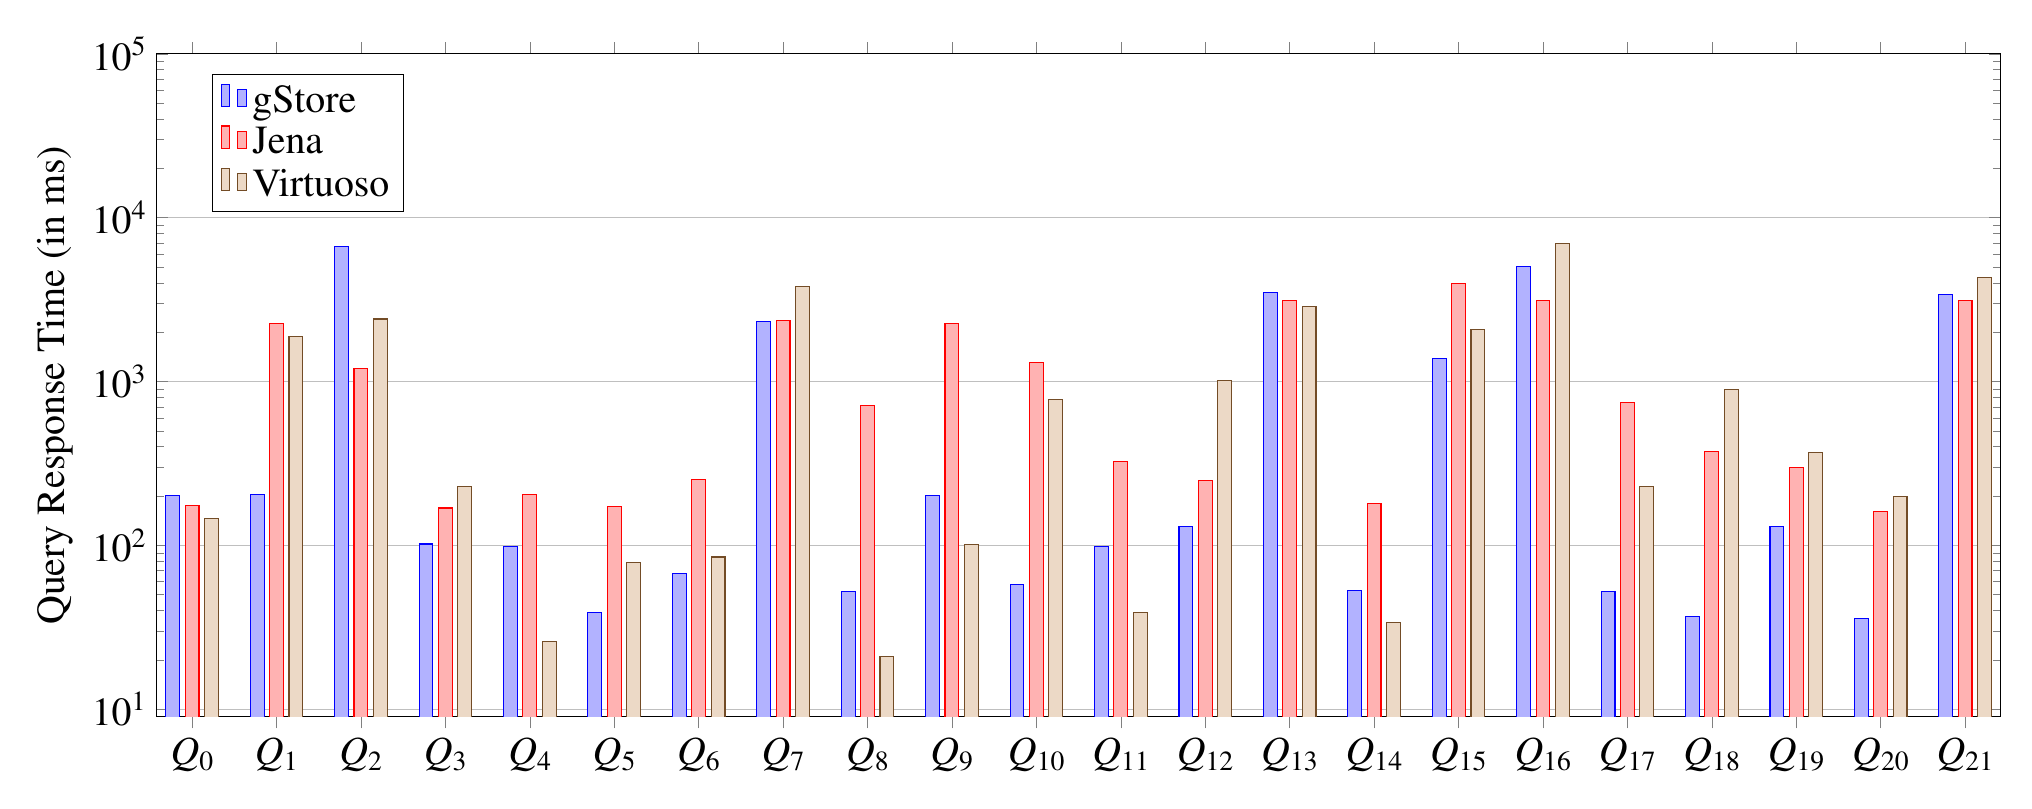
\begin{tikzpicture}[font=\Large]
 		 \begin{semilogyaxis}[
               width = 25cm,
               height = 10cm,
               ymax = 100000,
    			ybar,
   			ymajorgrids = true,
   			ylabel = {Query Response Time (in ms)},
                %xlabel = {Queries},
    			symbolic x coords = {$Q_{0}$,$Q_{1}$,$Q_{2}$,$Q_{3}$,$Q_{4}$,$Q_{5}$,$Q_{6}$,$Q_{7}$,$Q_{8}$,$Q_{9}$,$Q_{10}$,$Q_{11}$,$Q_{12}$,$Q_{13}$,$Q_{14}$,$Q_{15}$,$Q_{16}$,$Q_{17}$,$Q_{18}$,$Q_{19}$,$Q_{20}$,$Q_{21}$},
    bar width=5pt,
             enlarge x limits=0.02,
    			scaled y ticks = true,
			legend pos= north west,
 legend cell align=left
   		]
   \addplot coordinates {($Q_{0}$, 201) ($Q_{1}$, 204) ($Q_{2}$, 6688) ($Q_{3}$, 102) ($Q_{4}$, 98) ($Q_{5}$, 39) ($Q_{6}$, 67) ($Q_{7}$, 2327) ($Q_{8}$, 52) ($Q_{9}$, 202) ($Q_{10}$, 58) ($Q_{11}$, 98) ($Q_{12}$, 130) ($Q_{13}$, 3506) ($Q_{14}$, 53) ($Q_{15}$, 1379) ($Q_{16}$, 5049) ($Q_{17}$, 52) ($Q_{18}$, 37) ($Q_{19}$, 130) ($Q_{20}$, 36) ($Q_{21}$, 3396)};


\addplot coordinates {($Q_{0}$, 175) ($Q_{1}$, 2259) ($Q_{2}$, 1204) ($Q_{3}$, 169) ($Q_{4}$, 204) ($Q_{5}$, 172) ($Q_{6}$, 251) ($Q_{7}$, 2364) ($Q_{8}$, 718) ($Q_{9}$, 2253) ($Q_{10}$, 1308) ($Q_{11}$, 326) ($Q_{12}$, 248) ($Q_{13}$, 3125) ($Q_{14}$, 181) ($Q_{15}$, 3954) ($Q_{16}$, 3141) ($Q_{17}$, 748) ($Q_{18}$, 373) ($Q_{19}$, 298) ($Q_{20}$, 160) ($Q_{21}$, 3105)};

\addplot coordinates {($Q_{0}$, 146) ($Q_{1}$, 1890) ($Q_{2}$, 2409) ($Q_{3}$, 230) ($Q_{4}$, 26) ($Q_{5}$, 79) ($Q_{6}$, 85) ($Q_{7}$, 3800) ($Q_{8}$, 21) ($Q_{9}$, 101) ($Q_{10}$, 780) ($Q_{11}$, 39) ($Q_{12}$, 1020) ($Q_{13}$, 2877) ($Q_{14}$, 34) ($Q_{15}$, 2090) ($Q_{16}$, 6954) ($Q_{17}$, 230) ($Q_{18}$, 890) ($Q_{19}$, 370) ($Q_{20}$, 200) ($Q_{21}$, 4300)};

		
   		 \legend{gStore,Jena,Virtuoso}
  		\end{semilogyaxis}
\end{tikzpicture}

		}
		\label{fig:LUBM500Performance}%
	}
	\\
	\subfigure[LUBM 5000]{%
		\resizebox{0.98\columnwidth}{!}{
				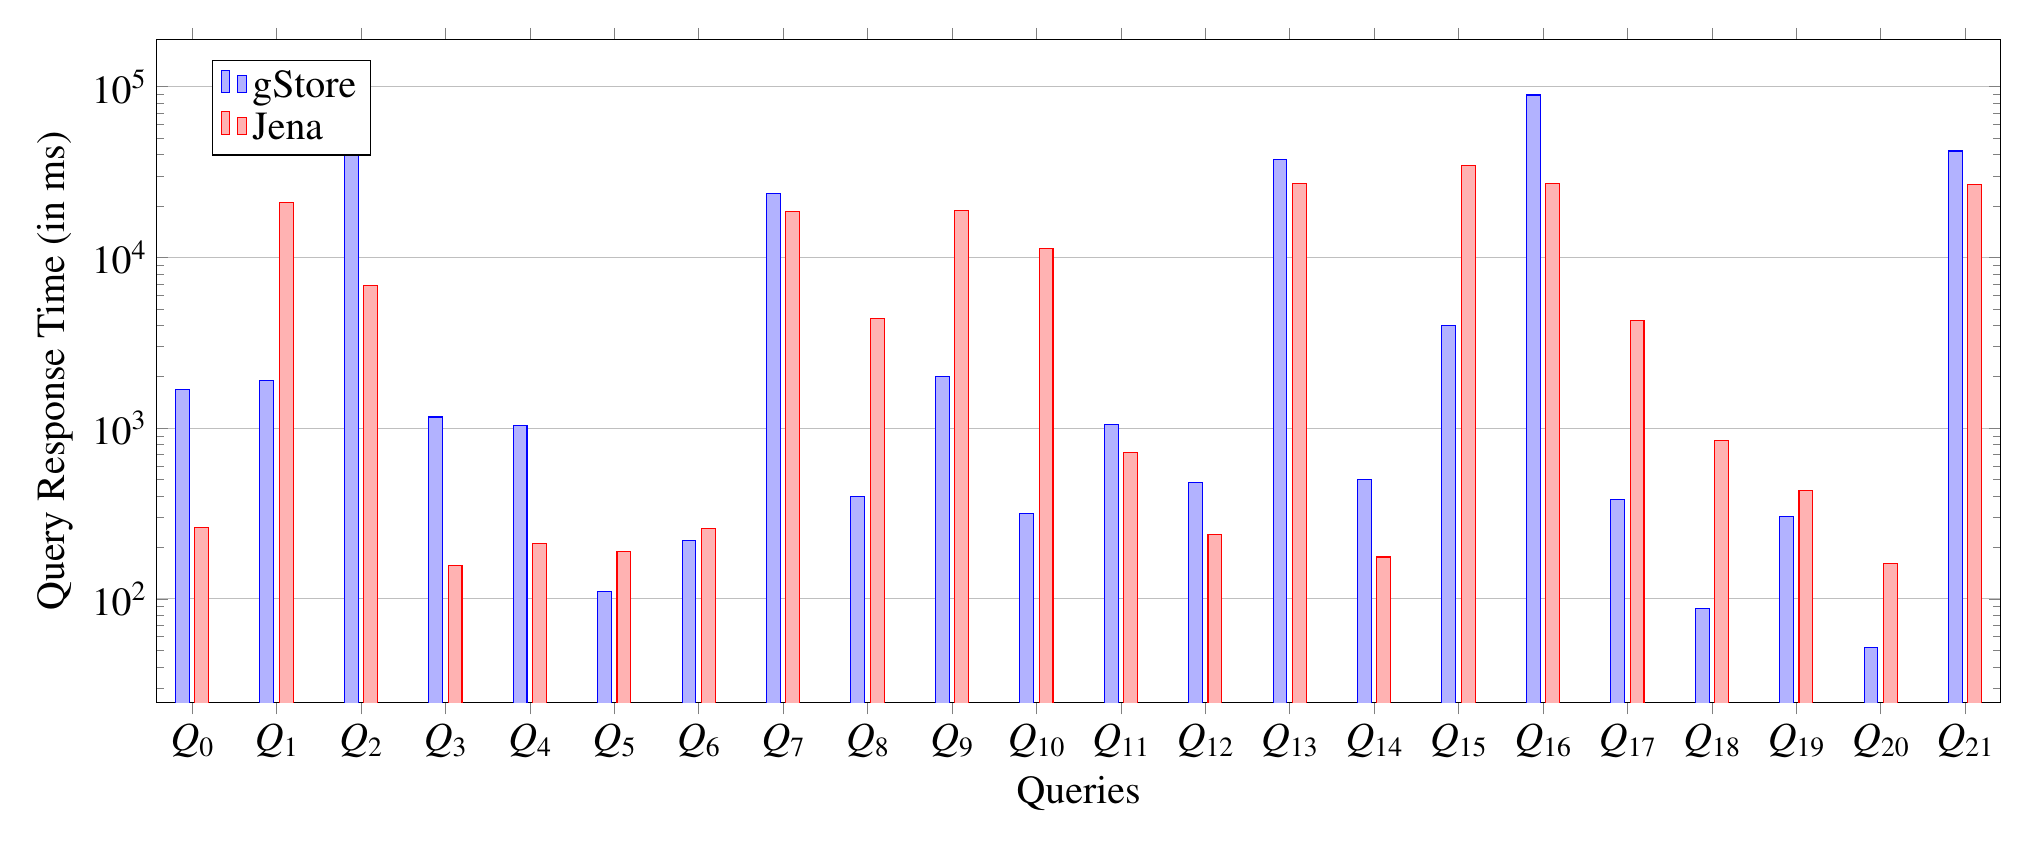
\begin{tikzpicture}[font=\Large]
 		 \begin{semilogyaxis}[
               width = 25cm,
               height = 10cm ,
    			ybar,
   			ymajorgrids = true,
   			ylabel = {Query Response Time (in ms)},
    			xlabel = {Queries},
    			symbolic x coords = {$Q_{0}$,$Q_{1}$,$Q_{2}$,$Q_{3}$,$Q_{4}$,$Q_{5}$,$Q_{6}$,$Q_{7}$,$Q_{8}$,$Q_{9}$,$Q_{10}$,$Q_{11}$,$Q_{12}$,$Q_{13}$,$Q_{14}$,$Q_{15}$,$Q_{16}$,$Q_{17}$,$Q_{18}$,$Q_{19}$,$Q_{20}$,$Q_{21}$},
    bar width=5pt,
             enlarge x limits=0.02,
    			scaled y ticks = true,
			legend pos= north west,
 legend cell align=left
   		]
   \addplot coordinates {($Q_{0}$, 1680) ($Q_{1}$, 1913) ($Q_{2}$, 69101) ($Q_{3}$, 1162) ($Q_{4}$, 1038) ($Q_{5}$, 110) ($Q_{6}$, 220) ($Q_{7}$, 23565) ($Q_{8}$, 398) ($Q_{9}$, 2000) ($Q_{10}$, 317) ($Q_{11}$, 1046) ($Q_{12}$, 483) ($Q_{13}$, 37581) ($Q_{14}$, 503) ($Q_{15}$, 4014) ($Q_{16}$, 89424) ($Q_{17}$, 381) ($Q_{18}$, 88) ($Q_{19}$, 304) ($Q_{20}$, 52) ($Q_{21}$, 42040)};


\addplot coordinates {($Q_{0}$, 262) ($Q_{1}$, 20865) ($Q_{2}$, 6814) ($Q_{3}$, 157) ($Q_{4}$, 212) ($Q_{5}$, 189) ($Q_{6}$, 257) ($Q_{7}$, 18469) ($Q_{8}$, 4365) ($Q_{9}$, 18933) ($Q_{10}$, 11305) ($Q_{11}$, 718) ($Q_{12}$, 237) ($Q_{13}$, 27059) ($Q_{14}$, 176) ($Q_{15}$, 34406) ($Q_{16}$, 26985) ($Q_{17}$, 4267) ($Q_{18}$, 845) ($Q_{19}$, 429) ($Q_{20}$, 162) ($Q_{21}$, 26853)};
		
   		 \legend{gStore,Jena}
  		\end{semilogyaxis}
\end{tikzpicture}

		}
		\label{fig:LUBM5000Performance}%
	}%
	\caption{Query Performance over LUBM}%
	\label{fig:LUBMPerformance}
\end{figure}

\begin{figure}[t]%
	\subfigure[WatDiv 10M]{%
		\resizebox{0.8\columnwidth}{!}{
				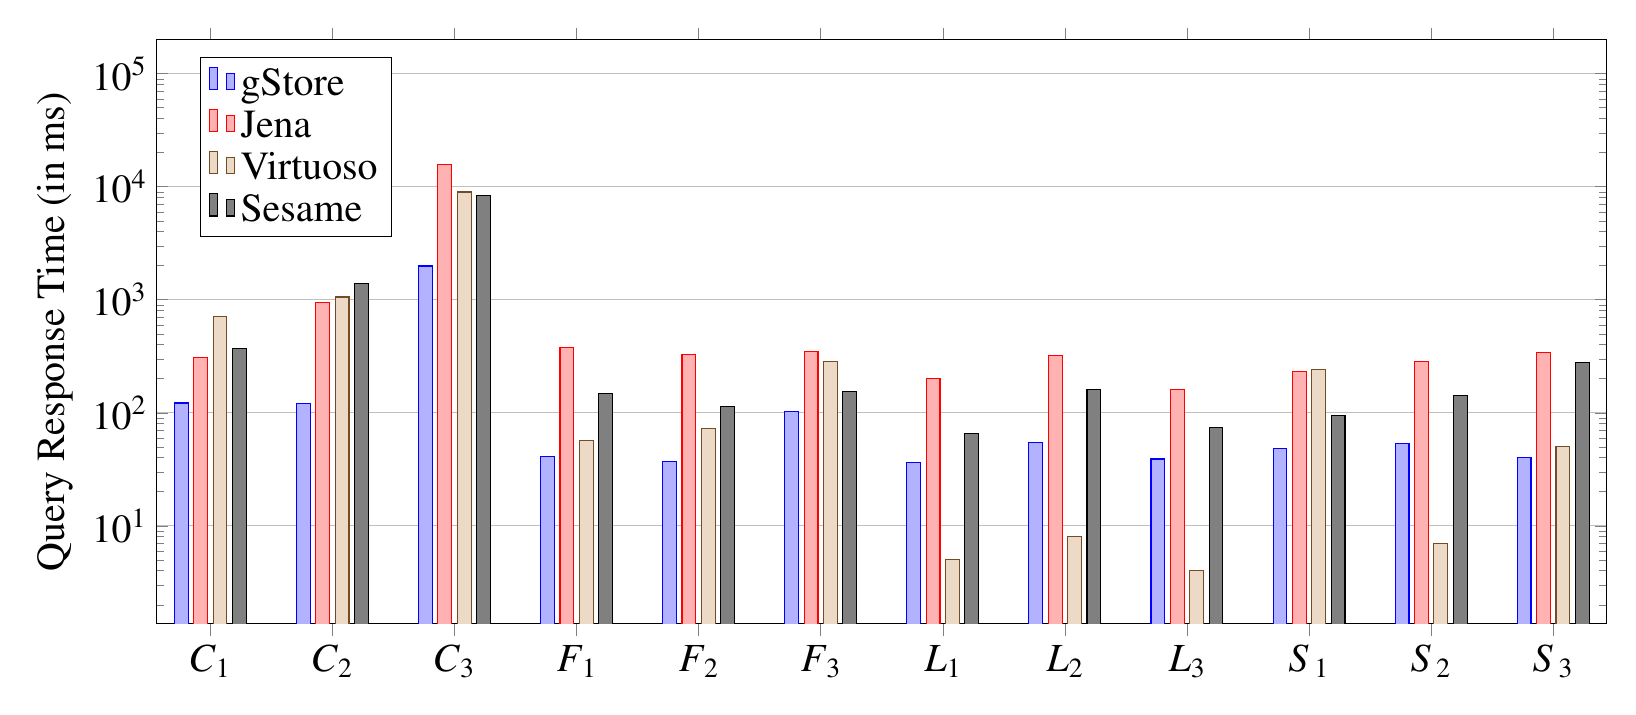
\begin{tikzpicture}[font=\Large]
 		 \begin{semilogyaxis}[
                width = 20cm,
               height = 9cm ,
               ymax=200000,
    			ybar,
   			ymajorgrids = true,
   			ylabel = {Query Response Time (in ms)},
                %xlabel = {Queries},
    			symbolic x coords = {$C_{1}$,$C_{2}$,$C_{3}$,$F_{1}$,$F_{2}$,$F_{3}$,$L_{1}$,$L_{2}$,$L_{3}$,$S_{1}$,$S_{2}$,$S_{3}$},
    bar width=5pt,
             enlarge x limits=0.04,
    			scaled y ticks = true,
			legend pos= north west,
 legend cell align=left
   		]
   \addplot coordinates {($C_{1}$, 122) ($C_{2}$, 121) ($C_{3}$, 1989) ($F_{1}$, 41) ($F_{2}$, 37) ($F_{3}$, 102) ($L_{1}$, 36) ($L_{2}$, 55) ($L_{3}$, 39) ($S_{1}$, 48) ($S_{2}$, 53) ($S_{3}$, 40)};


\addplot coordinates {($C_{1}$, 308) ($C_{2}$, 943) ($C_{3}$, 15805) ($F_{1}$, 375) ($F_{2}$, 327) ($F_{3}$, 346) ($L_{1}$, 202) ($L_{2}$, 322) ($L_{3}$, 162) ($S_{1}$, 230) ($S_{2}$, 283) ($S_{3}$, 344)};


\addplot coordinates {($C_{1}$, 715) ($C_{2}$, 1059) ($C_{3}$, 8987) ($F_{1}$, 57) ($F_{2}$, 73) ($F_{3}$, 283) ($L_{1}$, 5) ($L_{2}$, 8) ($L_{3}$, 4) ($S_{1}$, 242) ($S_{2}$, 7) ($S_{3}$, 50)};

\addplot coordinates {($C_{1}$, 368) ($C_{2}$, 1396) ($C_{3}$, 8312) ($F_{1}$, 148) ($F_{2}$, 114) ($F_{3}$, 154) ($L_{1}$, 66) ($L_{2}$, 160) ($L_{3}$, 74) ($S_{1}$, 95) ($S_{2}$, 143) ($S_{3}$, 279)};

		
   		 \legend{gStore,Jena,Virtuoso,Sesame}
  		\end{semilogyaxis}
\end{tikzpicture}

		}
		\label{fig:WatDiv10MPerformance}%
	}
	\subfigure[WatDiv 100M]{%
		\resizebox{0.8\columnwidth}{!}{
				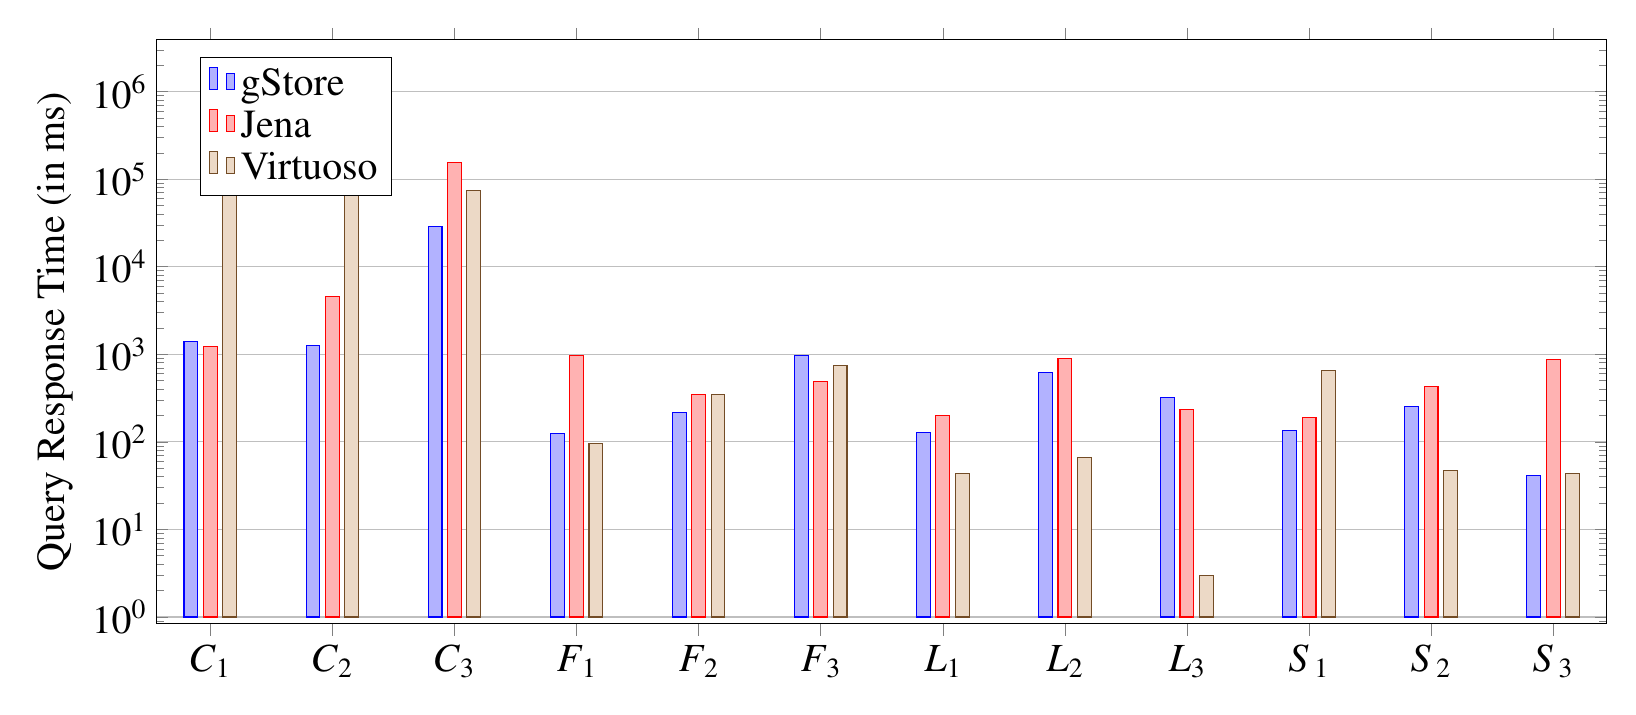
\begin{tikzpicture}[font=\Large]
 		 \begin{semilogyaxis}[
                width = 20cm,
               height = 9cm ,
    			ybar,
   			ymajorgrids = true,
   			ylabel = {Query Response Time (in ms)},
                %xlabel = {Queries},
    			symbolic x coords = {$C_{1}$,$C_{2}$,$C_{3}$,$F_{1}$,$F_{2}$,$F_{3}$,$L_{1}$,$L_{2}$,$L_{3}$,$S_{1}$,$S_{2}$,$S_{3}$},
    bar width=5pt,
             enlarge x limits=0.04,
    			scaled y ticks = true,
			legend pos= north west,
 legend cell align=left
   		]
   \addplot coordinates {($C_{1}$, 1408) ($C_{2}$, 1252) ($C_{3}$, 28677) ($F_{1}$, 126) ($F_{2}$, 215) ($F_{3}$, 971) ($L_{1}$, 129) ($L_{2}$, 623) ($L_{3}$, 321) ($S_{1}$, 135) ($S_{2}$, 253) ($S_{3}$, 41)};


\addplot coordinates {($C_{1}$, 1220) ($C_{2}$, 4617) ($C_{3}$, 153329) ($F_{1}$, 978) ($F_{2}$, 346) ($F_{3}$, 491) ($L_{1}$, 198) ($L_{2}$, 895) ($L_{3}$, 232) ($S_{1}$, 190) ($S_{2}$, 424) ($S_{3}$, 882)};


\addplot coordinates {($C_{1}$, 1087245) ($C_{2}$, 115820) ($C_{3}$, 74156) ($F_{1}$, 96) ($F_{2}$, 350) ($F_{3}$, 741) ($L_{1}$, 43) ($L_{2}$, 67) ($L_{3}$, 3) ($S_{1}$, 656) ($S_{2}$, 47) ($S_{3}$, 44)};

		
   		 \legend{gStore,Jena,Virtuoso}
  		\end{semilogyaxis}
\end{tikzpicture}

		}
		\label{fig:WatDiv100MPerformance}%
	}
	\subfigure[WatDiv 300M]{%
		\resizebox{0.8\columnwidth}{!}{
				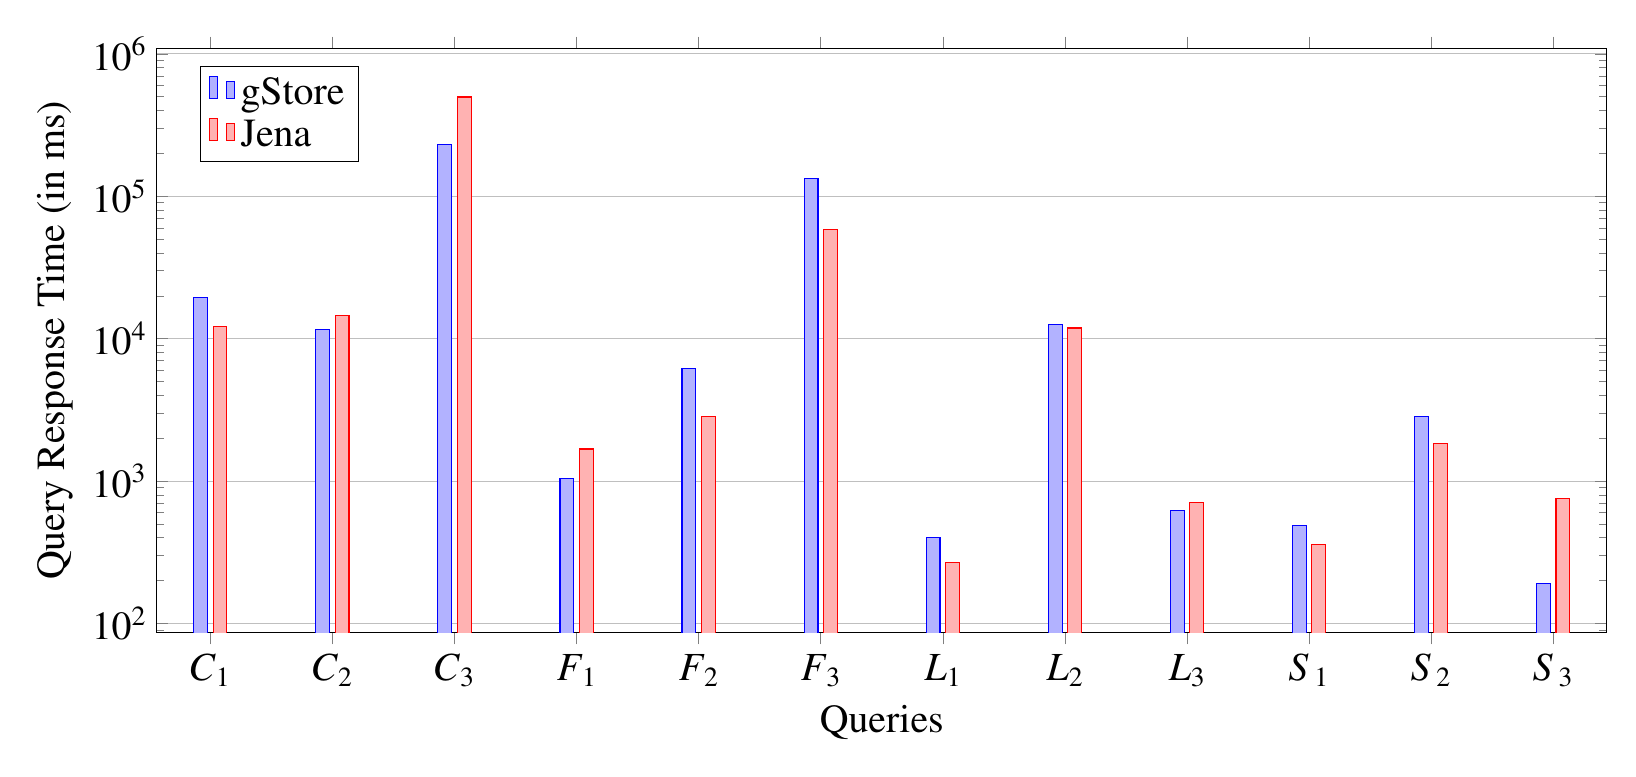
\begin{tikzpicture}[font=\Large]
 		 \begin{semilogyaxis}[
                width = 20cm,
               height = 9cm ,
    			ybar,
   			ymajorgrids = true,
   			ylabel = {Query Response Time (in ms)},
    			xlabel = {Queries},
    			symbolic x coords = {$C_{1}$,$C_{2}$,$C_{3}$,$F_{1}$,$F_{2}$,$F_{3}$,$L_{1}$,$L_{2}$,$L_{3}$,$S_{1}$,$S_{2}$,$S_{3}$},
    bar width=5pt,
             enlarge x limits=0.04,
    			scaled y ticks = true,
			legend pos= north west,
 legend cell align=left
   		]
   \addplot coordinates {($C_{1}$, 19602) ($C_{2}$, 11627) ($C_{3}$, 230831) ($F_{1}$, 1044) ($F_{2}$, 6194) ($F_{3}$, 134134) ($L_{1}$, 399) ($L_{2}$, 12548) ($L_{3}$, 620) ($S_{1}$, 490) ($S_{2}$, 2858) ($S_{3}$, 190)};


\addplot coordinates {($C_{1}$, 12241) ($C_{2}$, 14458) ($C_{3}$, 497314) ($F_{1}$, 1679) ($F_{2}$, 2844) ($F_{3}$, 58072) ($L_{1}$, 267) ($L_{2}$, 11884) ($L_{3}$, 711) ($S_{1}$, 359) ($S_{2}$, 1840) ($S_{3}$, 750)};

		
   		 \legend{gStore,Jena,Virtuoso}
  		\end{semilogyaxis}
\end{tikzpicture}

		}
		\label{fig:WatDiv300MPerformance}%
	}%
	\caption{Query Performance over WatDiv}%
	\label{fig:WatDivPerformance}
\end{figure}

\clearpage

\section{Comparative Analysis}

We can see that all query results of each database management system are matched through the result.log/, 
which means that the correctness of gStore is guaranteed. 

Both time cost and disk cost of gStore are higher than the others when analysing the load.log/,  
about one order of magnitude.  However, the size of the database generated by gStore can be reduced
because some files are useless(for example, six\_tuples).

By analysing the time.log/, we can discover that gStore performs better in very complicated SPARQL queries, 
for example, containing circles. However, for some queries which are in special structures(for example, 
star-shaped graph), the performance 
of gStore is worser than other RDF database management systems(for example, apache-jena).
These database management systems all performs well on small datasets. (query time usually less than 1s)

The memory cost is not counted concretely, but we can claim that the memory cost of gStore is just slightly 
higher than the others. As for disk cost, gStore is always larger, about one order of magnitude.

All datasets and queries we used are listed in this document, to provide a more thorough understanding of 
the experiment results.

Below is for the WatDiv datasets, and the corresponding queries are placed in \hyperref[watdiv]{WatDiv Queries}.

\begin{table}[htbp]
	\centering
	\begin{tabular}{p{60pt}>{\centering}p{60pt}>{\raggedleft\arraybackslash}p{60pt}>{\raggedleft\arraybackslash}p{60pt}>{\raggedleft\arraybackslash}p{60pt}>{\raggedleft\arraybackslash}p{60pt}}
		\toprule
		Dataset & Size & Triple & Predicate & Entity & Literal \\
		\midrule
		watdiv\_100M & 15599074048 & 108997714 & 86 & 5212745 & 5038202 \\
		watdiv\_10M & 1542624409 & 10916457 & 86 & 521945 & 530626 \\
		watdiv\_200 & 3138192889 & 20014680 & 86 & 1043145 & 1046759 \\
		watdiv\_300M & 47670221085 & 329539576 & 86 & 15636745 & 14749420 \\
		watdiv\_500 & 7858764942 & 54905597 & 86 & 2606745 & 2571173 \\
		\bottomrule
	\end{tabular}
	\caption{WatDiv series}
\end{table}

\clearpage

For WatDiv datasets, gStore performs worser in F3.sql. The reason is that all vertices are filtered by VSTree, but the candidate num 
is still very large. There are many edges in F3.sql, so the cost of join process can be very high. \\

Below is for the LUBM datasets, and the corresponding queries are placed in \hyperref[lubm]{LUBM Queries}.

\begin{table}[htbp]
	\centering
	\begin{tabular}{p{60pt}>{\centering}p{60pt}>{\raggedleft\arraybackslash}p{60pt}>{\raggedleft\arraybackslash}p{60pt}>{\raggedleft\arraybackslash}p{60pt}>{\raggedleft\arraybackslash}p{60pt}}
		\toprule
		Dataset & Size & Triple & Predicate & Entity & Literal \\
		\midrule
		lubm\_10 & 11835527 & 99550 & 28413 & 17 & 0 \\
		lubm\_5000 & 8134671485 & 66718642 & 17 & 16437950 & 0 \\
		lubm\_500 & 801112089 & 6652613 & 17 & 1648692 & 0 \\
		\bottomrule
	\end{tabular}
	\caption{LUBM series}
\end{table}

For LUBM datasets, gStore performs worser in q0.sql, q13.sql, q16.sql, q21.sql, q2.sql, q3.sql, q4.sql and q7.sql. 
We can discover that in star-shaped query graph, the satellite vertices should not be filtered by VSTree. 
In addition, if there is only one triple in the query graph, none should be put into the VSTree. \\

Below is for the BSBM datasets, and the corresponding queries are placed in \hyperref[bsbm]{BSBM Queries}.

\begin{table}[htbp]
	\centering
	\begin{tabular}{p{60pt}>{\centering}p{60pt}>{\raggedleft\arraybackslash}p{60pt}>{\raggedleft\arraybackslash}p{60pt}>{\raggedleft\arraybackslash}p{60pt}>{\raggedleft\arraybackslash}p{60pt}}
		\toprule
		Dataset & Size & Triple & Predicate & Entity & Literal \\
		\midrule
		bsbm\_100000 & 9100827924 & 34872182 & 40 & 5207266 & 3678812 \\
		bsbm\_10000 & 912646084 & 3534773 & 40 & 526590 & 480970 \\
		bsbm\_1000 & 95077406 & 371911 & 40 & 56487 & 60239 \\
		bsbm\_100 & 10174119 & 40177 & 40 & 6197 & 8008 \\
		bsbm\_500 & 48548941 & 190496 & 40 & 28712 & 31956 \\
		\bottomrule
	\end{tabular}
	\caption{BSBM series}
\end{table}

\clearpage

For BSBM datasets, gStore performs worser in self1.sql. 
In this case, we had better get the result by using a p2so index, which is implemented by B+ tree.
If using VSTree here, the cost of filter process is high due to large data size(more precisely, the candidate size after VSTree is very large), and the cost of 
join process may be higher. \\

Below is for the DBpedia datasets, and the corresponding queries are placed in \hyperref[dbpedia]{DBpedia Queries}.

\begin{table}[htbp]
	\centering
	\begin{tabular}{p{60pt}>{\centering}p{60pt}>{\raggedleft\arraybackslash}p{60pt}>{\raggedleft\arraybackslash}p{60pt}>{\raggedleft\arraybackslash}p{60pt}>{\raggedleft\arraybackslash}p{60pt}}
		\toprule
		Dataset & Size & Triple & Predicate & Entity & Literal \\
		\midrule
		dbpedia2014 & 23844158944 & 170784508 & 57354 & 7123915 & 14971449 \\
		\bottomrule
	\end{tabular}
	\caption{DBpedia series}
\end{table}

For DBpedia datasets, gStore performs worser in q3.sql, q4.sql and q5.sql. The reason is almost the same
as others. \\

\clearpage

\section{Conclusion}

gStore can go well with RDF datasets which are in N-Triples format, while the other database
management systems may come across some questions. In addition, gStore outperforms other systems
on very complicated SPARQL queries. What is more, gStore is highly extensively because it uses graph model
instead of relational model. \\

However, there are also some shortcomings for gStore:
\begin{enumerate}
	\item RDF datasets in XML format are not supported
	\item the memory and disk cost is high
	\item only select-where clause can be used in SPARQL queries
	\item unbounded predicates can not be contained in queries
	\item too much warnnings when compiling the project(especially redefine warning)
	\item gStore is not always more efficient than other database management systems
\end{enumerate}

\clearpage

\section{Prospective}

Out of question, the performance of gStore can be improved a lot later. 
The future work is listed below:
\begin{enumerate}
	\item fix/add datasets and corresponding queries 
	\item support queries which are not in BGP(Basic Graph Pattern) efficiently
	\item improve the encoding method in Signature/ and VSTree/
	\item adjust the query plan, not always using VSTree as filter
\end{enumerate}

\clearpage

\section{Appendix}

%\begin{comment}
%\begin{lstlisting}[language={[ANSI]C},numbers=left,numberstyle=\tiny,keywordstyle=\color{blue!70},commentstyle=\color{red!50!green!50!blue!50},frame=shadowbox, rulesepcolor=\color{red!20!green!20!blue!20}] 
%	int main(int argc, char ** argv) 
%	{ 
%		
%		printf("Hello world! \n"); 
%		return 0; 
%	} 
%\end{lstlisting}


\subsection{WatDiv queries}\label{watdiv}

\subsubsection{C1.sql}

\begin{lstlisting}[language=SQL] 
SELECT ?v0 ?v4 ?v6 ?v7 WHERE 
{
	?v0 <http://schema.org/caption> ?v1 .
	?v0 <http://schema.org/text> ?v2 .
	?v0 <http://schema.org/contentRating> ?v3 .
	?v0 <http://purl.org/stuff/rev#hasReview> ?v4 .
	?v4 <http://purl.org/stuff/rev#title> ?v5 .
	?v4 <http://purl.org/stuff/rev#reviewer> ?v6 .
	?v7 <http://schema.org/actor> ?v6 .
	?v7 <http://schema.org/language> ?v8 .
}
\end{lstlisting} 

\subsubsection{C2.sql}

\begin{lstlisting}[language=SQL] 
SELECT ?v0 ?v3 ?v4 ?v8 WHERE 
{
	?v0 <http://schema.org/legalName> ?v1 .
	?v0 <http://purl.org/goodrelations/offers> ?v2 .
	?v2 <http://schema.org/eligibleRegion> <http://db.uwaterloo.ca/~galuc/wsdbm/Country5> .
	?v2 <http://purl.org/goodrelations/includes> ?v3 .
	?v4 <http://schema.org/jobTitle> ?v5 .
	?v4 <http://xmlns.com/foaf/homepage> ?v6 .
	?v4 <http://db.uwaterloo.ca/~galuc/wsdbm/makesPurchase> ?v7 .
	?v7 <http://db.uwaterloo.ca/~galuc/wsdbm/purchaseFor> ?v3 .
	?v3 <http://purl.org/stuff/rev#hasReview> ?v8 .
	?v8 <http://purl.org/stuff/rev#totalVotes> ?v9 .
}
\end{lstlisting}

\subsubsection{C3.sql}

\begin{lstlisting}[language=SQL] 
SELECT ?v0 WHERE 
{
	?v0 <http://db.uwaterloo.ca/~galuc/wsdbm/likes> ?v1 .
	?v0 <http://db.uwaterloo.ca/~galuc/wsdbm/friendOf> ?v2 .
	?v0 <http://purl.org/dc/terms/Location> ?v3 .
	?v0 <http://xmlns.com/foaf/age> ?v4 .
	?v0 <http://db.uwaterloo.ca/~galuc/wsdbm/gender> ?v5 .
	?v0 <http://xmlns.com/foaf/givenName> ?v6 .
}
\end{lstlisting}

\subsubsection{F1.sql}

\begin{lstlisting}[language=SQL] 
SELECT ?v0 ?v2 ?v3 ?v4 ?v5 WHERE 
{
	?v0 <http://ogp.me/ns#tag> <http://db.uwaterloo.ca/~galuc/wsdbm/Topic103> .
	?v0 <http://www.w3.org/1999/02/22-rdf-syntax-ns#type> ?v2 .
	?v3 <http://schema.org/trailer> ?v4 .
	?v3 <http://schema.org/keywords> ?v5 .
	?v3 <http://db.uwaterloo.ca/~galuc/wsdbm/hasGenre> ?v0 .
	?v3 <http://www.w3.org/1999/02/22-rdf-syntax-ns#type> <http://db.uwaterloo.ca/~galuc/wsdbm/ProductCategory2> .
}
\end{lstlisting}

\subsubsection{F2.sql}

\begin{lstlisting}[language=SQL] 
SELECT ?v0 ?v1 ?v2 ?v4 ?v5 ?v6 ?v7 WHERE 
{
	?v0 <http://xmlns.com/foaf/homepage> ?v1 .
	?v0 <http://ogp.me/ns#title> ?v2 .
	?v0 <http://www.w3.org/1999/02/22-rdf-syntax-ns#type> ?v3 .
	?v0 <http://schema.org/caption> ?v4 .
	?v0 <http://schema.org/description> ?v5 .
	?v1 <http://schema.org/url> ?v6 .
	?v1 <http://db.uwaterloo.ca/~galuc/wsdbm/hits> ?v7 .
	?v0 <http://db.uwaterloo.ca/~galuc/wsdbm/hasGenre> <http://db.uwaterloo.ca/~galuc/wsdbm/SubGenre35> .
}
\end{lstlisting}

\subsubsection{F3.sql}

\begin{lstlisting}[language=SQL] 
SELECT ?v0 ?v1 ?v2 ?v4 ?v5 ?v6 WHERE 
{
	?v0 <http://schema.org/contentRating> ?v1 .
	?v0 <http://schema.org/contentSize> ?v2 .
	?v0 <http://db.uwaterloo.ca/~galuc/wsdbm/hasGenre> <http://db.uwaterloo.ca/~galuc/wsdbm/SubGenre59> .
	?v4 <http://db.uwaterloo.ca/~galuc/wsdbm/makesPurchase> ?v5 .
	?v5 <http://db.uwaterloo.ca/~galuc/wsdbm/purchaseDate> ?v6 .
	?v5 <http://db.uwaterloo.ca/~galuc/wsdbm/purchaseFor> ?v0 .
}
\end{lstlisting}

\subsubsection{L1.sql}

\begin{lstlisting}[language=SQL] 
SELECT ?v0 ?v2 ?v3 WHERE 
{
	?v0 <http://db.uwaterloo.ca/~galuc/wsdbm/subscribes> <http://db.uwaterloo.ca/~galuc/wsdbm/Website38303> .
	?v2 <http://schema.org/caption> ?v3 .
	?v0 <http://db.uwaterloo.ca/~galuc/wsdbm/likes> ?v2 .
}
\end{lstlisting}

\subsubsection{L2.sql}

\begin{lstlisting}[language=SQL] 
SELECT ?v1 ?v2 WHERE 
{
	<http://db.uwaterloo.ca/~galuc/wsdbm/City131> <http://www.geonames.org/ontology#parentCountry> ?v1 .
	?v2 <http://db.uwaterloo.ca/~galuc/wsdbm/likes> <http://db.uwaterloo.ca/~galuc/wsdbm/Product0> .
	?v2 <http://schema.org/nationality> ?v1 .
}
\end{lstlisting}

\subsubsection{L3.sql}

\begin{lstlisting}[language=SQL]
SELECT ?v0 ?v1 WHERE 
{
	?v0 <http://db.uwaterloo.ca/~galuc/wsdbm/likes> ?v1 .
	?v0 <http://db.uwaterloo.ca/~galuc/wsdbm/subscribes> <http://db.uwaterloo.ca/~galuc/wsdbm/Website20769> .
}
\end{lstlisting}

\subsubsection{S1.sql}

\begin{lstlisting}[language=SQL]
SELECT ?v0 ?v1 ?v3 ?v4 ?v5 ?v6 ?v7 ?v8 ?v9 WHERE 
{
	?v0 <http://purl.org/goodrelations/includes> ?v1 .
	<http://db.uwaterloo.ca/~galuc/wsdbm/Retailer391> <http://purl.org/goodrelations/offers> ?v0 .
	?v0 <http://purl.org/goodrelations/price> ?v3 .
	?v0 <http://purl.org/goodrelations/serialNumber> ?v4 .
	?v0 <http://purl.org/goodrelations/validFrom> ?v5 .
	?v0 <http://purl.org/goodrelations/validThrough> ?v6 .
	?v0 <http://schema.org/eligibleQuantity> ?v7 .
	?v0 <http://schema.org/eligibleRegion> ?v8 .
	?v0 <http://schema.org/priceValidUntil> ?v9 .
}
\end{lstlisting}

\subsubsection{S2.sql}

\begin{lstlisting}[language=SQL]
SELECT ?v0 ?v1 ?v3 WHERE 
{
	?v0 <http://purl.org/dc/terms/Location> ?v1 .
	?v0 <http://schema.org/nationality> <http://db.uwaterloo.ca/~galuc/wsdbm/Country23> .
	?v0 <http://db.uwaterloo.ca/~galuc/wsdbm/gender> ?v3 .
	?v0 <http://www.w3.org/1999/02/22-rdf-syntax-ns#type> <http://db.uwaterloo.ca/~galuc/wsdbm/Role2> .
}
\end{lstlisting}

\subsubsection{S3.sql}

\begin{lstlisting}[language=SQL]
SELECT ?v0 ?v2 ?v3 ?v4 WHERE 
{
	?v0 <http://www.w3.org/1999/02/22-rdf-syntax-ns#type> <http://db.uwaterloo.ca/~galuc/wsdbm/ProductCategory12> .
	?v0 <http://schema.org/caption> ?v2 .
	?v0 <http://db.uwaterloo.ca/~galuc/wsdbm/hasGenre> ?v3 .
	?v0 <http://schema.org/publisher> ?v4 .
}
\end{lstlisting}

\subsection{LUBM queries}\label{lubm}

\subsubsection{q0.sql}

\begin{lstlisting}[language=SQL] 
select ?x where
{
	?x      <ub:name>       <FullProfessor0>.
}
\end{lstlisting}

\subsubsection{q1.sql}

\begin{lstlisting}[language=SQL]
select ?x where
{
	?x      <rdf:type>      <ub:GraduateStudent>.
	?y      <rdf:type>      <ub:University>.
	?z      <rdf:type>      <ub:Department>.
	?x      <ub:memberOf>   ?z.
	?z      <ub:subOrganizationOf>  ?y.
	?x      <ub:undergraduateDegreeFrom>    ?y.
}
\end{lstlisting}

\subsubsection{q2.sql}

\begin{lstlisting}[language=SQL]
select ?x where
{
	?x      <rdf:type>      <ub:Course>.
	?x      <ub:name>       ?y.
}  
\end{lstlisting}

\subsubsection{q3.sql}

\begin{lstlisting}[language=SQL]
select ?x where
{
	?x      <rdf:type>      <ub:UndergraduateStudent>.
	?y      <rdf:type>      <ub:University>.
	?z      <rdf:type>      <ub:Department>.
	?x      <ub:memberOf>   ?z.
	?z      <ub:subOrganizationOf>  ?y.
	?x      <b:undergraduateDegreeFrom>     ?y.
}
\end{lstlisting}

\subsubsection{q4.sql}

\begin{lstlisting}[language=SQL]
elect ?x ?y1 ?y2 ?y3 where
{
	?x      <ub:worksFor>   <http://www.Department0.University0.edu>.
	?x      <rdf:type>      <ub:FullProfessor>.
	?x      <ub:name>       ?y1.
	?x      <ub:emailAddress>       ?y2.
	?x      <ub:telephone>  ?y3.
}
\end{lstlisting}

\subsubsection{q5.sql}

\begin{lstlisting}[language=SQL]
select ?x where
{
	?x      <ub:subOrganizationOf>  <http://www.Department0.University0.edu>.
	?x      <rdf:type>      <ub:ResearchGroup>.
}
\end{lstlisting}

\subsubsection{q6.sql}

\begin{lstlisting}[language=SQL]
select ?x ?y where
{
	?y      <ub:subOrganizationOf>  <http://www.University0.edu>.
	?y      <rdf:type>      <ub:Department>.
	?x      <ub:worksFor>   ?y.
	?x      <rdf:type>      <ub:FullProfessor>.
}
\end{lstlisting}

\subsubsection{q7.sql}

\begin{lstlisting}[language=SQL]
select ?x ?y ?z where
{
	?x      <rdf:type>      <ub:UndergraduateStudent>.
	?y      <rdf:type>      <ub:FullProfessor>.
	?z      <rdf:type>      <ub:Course>.
	?x      <ub:advisor>    ?y.
	?x      <ub:takesCourse>        ?z.
	?y      <ub:teacherOf>  ?z.
}
\end{lstlisting}

\subsubsection{q8.sql}

\begin{lstlisting}[language=SQL]
select ?X where
{
	?X      <rdf:type>      <ub:GraduateStudent>.
	?X      <ub:takesCourse>        <http://www.Department0.University0.edu/GraduateCourse0>.
}
\end{lstlisting}

\subsubsection{q9.sql}

\begin{lstlisting}[language=SQL]
select ?X ?Y ?Z where
{
	?X      <rdf:type>      <ub:GraduateStudent>.
	?Y      <rdf:type>      <ub:University>.
	?Z      <rdf:type>      <ub:Department>.
	?X      <ub:memberOf>   ?Z.
	?Z      <ub:subOrganizationOf>  ?Y.
	?X      <ub:undergraduateDegreeFrom>    ?Y.
}    
\end{lstlisting}

\subsubsection{q10.sql}

\begin{lstlisting}[language=SQL]
select ?X where
{
	?X      <rdf:type>      <ub:Publication>.
	?X      <ub:publicationAuthor>  <http://www.Department0.University0.edu/AssistantProfessor0>.
}
\end{lstlisting}

\subsubsection{q11.sql}

\begin{lstlisting}[language=SQL]
select ?Y1 ?Y2 ?Y3 where
{
	?X      <rdf:type>      <ub:FullProfessor>.
	?X      <ub:worksFor>   <http://www.Department0.University0.edu>.
	?X      <ub:name>       ?Y1.
	?X      <ub:emailAddress>       ?Y2.
	?X      <ub:telephone>  ?Y3.
}
\end{lstlisting}

\subsubsection{q12.sql}

\begin{lstlisting}[language=SQL]
select ?X where
{
	?X      <ub:memberOf>   <http://www.Department0.University0.edu>.
}
\end{lstlisting}

\subsubsection{q13.sql}

\begin{lstlisting}[language=SQL]
select ?X where
{
	?X      <rdf:type>      <ub:UndergraduateStudent>.
}
\end{lstlisting}

\subsubsection{q14.sql}

\begin{lstlisting}[language=SQL]
elect ?X ?Y where
{
	?X      <rdf:type>      <ub:Student>.
	?Y      <rdf:type>      <ub:Course>.
	?X      <ub:takesCourse>        ?Y.
	<http://www.Department0.University0.edu/AssociateProfessor0>    <ub:teacherOf>  ?Y.
}
\end{lstlisting}

\subsubsection{q15.sql}

\begin{lstlisting}[language=SQL]
select ?X where
{
	?X      <rdf:type>      <ub:UndergraduateStudent>.
	?Y      <rdf:type>      <ub:Department>.
	?X      <ub:memberOf>   ?Y.
	?Y      <ub:subOrganizationOf>  <http://www.University0.edu>.
	?X      <ub:emailAddress>       ?Z.
}
\end{lstlisting}

\subsubsection{q16.sql}

\begin{lstlisting}[language=SQL]
select ?X ?Y ?Z where
{
	?X      <rdf:type>      <ub:UndergraduateStudent>.
	?Z      <rdf:type>      <ub:Course>.
	?X      <ub:advisor>    ?Y.
	?Y      <ub:teacherOf>  ?Z.
	?X      <ub:takesCourse>        ?Z.
}
\end{lstlisting}

\subsubsection{q17.sql}

\begin{lstlisting}[language=SQL]
select ?X where
{
	?X      <rdf:type>      <ub:GraduateStudent>.
	?X      <ub:takesCourse>        <http://www.Department0.University0.edu/GraduateCourse0>.
}
\end{lstlisting}

\subsubsection{q18.sql}

\begin{lstlisting}[language=SQL]
select ?X where
{
	?X      <rdf:type>      <ub:ResearchGroup>.
	?X      <ub:subOrganizationOf>  <http://www.University0.edu>.
}
\end{lstlisting}

\subsubsection{q19.sql}

\begin{lstlisting}[language=SQL]
select ?X ?Y where
{
	?Y      <rdf:type>      <ub:Department>.
	?X      <ub:worksFor>   ?Y.
	?Y      <ub:subOrganizationOf>  <http://www.University0.edu>.
}
\end{lstlisting}

\subsubsection{q20.sql}

\begin{lstlisting}[language=SQL]
select ?X where
{
	<http://www.University0.edu>    <ub:undergraduateDegreeFrom>    ?X.
}
\end{lstlisting}

\subsubsection{q21.sql}

\begin{lstlisting}[language=SQL]
select ?X where
{
	?X      <rdf:type>      <ub:UndergraduateStudent>.
}
\end{lstlisting}

\subsection{BSBM queries}\label{bsbm}

\subsubsection{self0.sql}

\begin{lstlisting}[language=SQL] 
select ?v0 where
{
	?v0 <http://www4.wiwiss.fu-berlin.de/bizer/bsbm/v01/vocabulary/rating2> "6"^^<http://www.w3.org/2001/XMLSchema#integer> .
}
\end{lstlisting}

\subsubsection{self1.sql}

\begin{lstlisting}[language=SQL] 
select ?v0 ?v1 where
{
	?v0 <http://www.w3.org/1999/02/22-rdf-syntax-ns#type> ?v1 .
}
\end{lstlisting}

\subsubsection{self2.sql}

\begin{lstlisting}[language=SQL] 
select ?v0 ?v1 where
{
	?v0 <http://www.w3.org/2000/01/rdf-schema#label> ?v1 .
	?v1 <http://purl.org/dc/elements/1.1/publisher> ?v2 .
}
\end{lstlisting}

\subsubsection{self3.sql}

\begin{lstlisting}[language=SQL] 
select ?v0 ?v1 ?v2 where
{
	?v0 <http://purl.org/dc/elements/1.1/publisher> ?v1 .
	?v0 <http://purl.org/dc/elements/1.1/date> ?v2 .
}
\end{lstlisting}

\subsubsection{self4.sql}

\begin{lstlisting}[language=SQL] 
select ?v0 ?v1 ?v2 where
{
	?v0 <http://www.w3.org/2000/01/rdf-schema#label> ?v2 .
	?v1 <http://www.w3.org/2000/01/rdf-schema#subClassOf> ?v2 .
}
\end{lstlisting}

\subsubsection{self5.sql}

\begin{lstlisting}[language=SQL] 
select ?v0 ?v1 ?v2 ?v3 where
{
	?v0 <http://www.w3.org/2000/01/rdf-schema#label> ?v1 .
	?v0 <http://www.w3.org/1999/02/22-rdf-syntax-ns#type> ?v2 .
	?v3 <http://www.w3.org/2000/01/rdf-schema#label> ?v1 .
	?v3 <http://purl.org/dc/elements/1.1/publisher> <http://www4.wiwiss.fu-berlin.de/bizer/bsbm/v01/instances/StandardizationInstitution1> .
}
\end{lstlisting}

\subsubsection{self6.sql}

\begin{lstlisting}[language=SQL] 
select ?v0 ?v1 ?v2 ?v3 ?v4 where
{
	?v0 <http://www.w3.org/1999/02/22-rdf-syntax-ns#type> ?v1 .
	?v0 <http://purl.org/dc/elements/1.1/date> ?v2 .
	?v3 <http://www.w3.org/2000/01/rdf-schema#comment> ?v4 .
	<http://www4.wiwiss.fu-berlin.de/bizer/bsbm/v01/instances/ProductType2> <http://www.w3.org/2000/01/rdf-schema#comment> ?v4 .
	?v3 <http://www.w3.org/1999/02/22-rdf-syntax-ns#type> ?v1 .
}
\end{lstlisting}

\subsubsection{self7.sql}

\begin{lstlisting}[language=SQL] 
select ?v0 ?v1 ?v2 ?v3 ?v4 where
{
	?v0 <http://purl.org/dc/elements/1.1/title> ?v1 .
	?v0 <http://purl.org/dc/elements/1.1/publisher> <http://www4.wiwiss.fu-berlin.de/bizer/bsbm/v01/instances/dataFromRatingSite11/RatingSite11> .
	?v0 <http://purl.org/stuff/rev#text> ?v4 .
	?v2 <http://purl.org/stuff/rev#reviewer> ?v3 .
	?v2 <http://purl.org/dc/elements/1.1/date> "2008-04-16"^^<http://www.w3.org/2001/XMLSchema#date> .
	?v2 <http://purl.org/stuff/rev#text> ?v4
}
\end{lstlisting}

\subsubsection{self8.sql}

\begin{lstlisting}[language=SQL] 
select ?v0 ?v1 ?v2 ?v3 ?v4 ?v5 ?v6 where
{
	?v0 <http://www.w3.org/2000/01/rdf-schema#subClassOf> ?v1 .
	?v0 <http://purl.org/dc/elements/1.1/date> ?v2 .
	?v3 <http://purl.org/dc/elements/1.1/publisher> ?v4 .
	?v3 <http://www.w3.org/2000/01/rdf-schema#subClassOf> ?v1 .
	?v5 <http://purl.org/dc/elements/1.1/publisher> ?v6 .
	?v5 <http://purl.org/dc/elements/1.1/date> ?v2 .
}
\end{lstlisting}

\subsubsection{self9.sql}

\begin{lstlisting}[language=SQL] 
select ?v0 ?v1 ?v2 ?v3 ?v4 ?v5 ?v6 ?v7 ?v8 where
{
	?v0 <http://purl.org/dc/elements/1.1/date> "2000-07-17"^^<http://www.w3.org/2001/XMLSchema#date> .
	?v0 <http://purl.org/dc/elements/1.1/publisher> ?v1 .
	?v0 <http://www.w3.org/2000/01/rdf-schema#label> ?v2 .
	?v0 <http://www.w3.org/2000/01/rdf-schema#comment> ?v8 .
	?v3 <http://www.w3.org/2000/01/rdf-schema#subClassOf> <http://www4.wiwiss.fu-berlin.de/bizer/bsbm/v01/instances/ProductType2> .
	?v3 <http://purl.org/dc/elements/1.1/publisher> ?v1 .
	?v3 <http://www.w3.org/2000/01/rdf-schema#label> ?v4 .
	?v3 <http://www.w3.org/1999/02/22-rdf-syntax-ns#type> ?v7 .
	?v5 <http://www.w3.org/2000/01/rdf-schema#label> ?v2 .
	?v5 <http://purl.org/dc/elements/1.1/publisher> ?v6 .
	?v5 <http://www.w3.org/1999/02/22-rdf-syntax-ns#type> ?v7 .
}
\end{lstlisting}

\subsection{DBpedia queries}\label{dbpedia}

\subsubsection{q0.sql}

\begin{lstlisting}[language=SQL] 
select ?v0 where
{
	?v0 <http://www.w3.org/1999/02/22-rdf-syntax-ns#type> <http://dbpedia.org/class/yago/LanguagesOfBotswana> .
	?v0 <http://www.w3.org/1999/02/22-rdf-syntax-ns#type>    <http://dbpedia.org/class/yago/LanguagesOfNamibia> .
	?v0 <http://www.w3.org/1999/02/22-rdf-syntax-ns#type> <http://dbpedia.org/ontology/Language> .
}
\end{lstlisting}

\subsubsection{q1.sql}

\begin{lstlisting}[language=SQL] 
select ?v0 where
{
	?v0 <http://dbpedia.org/ontology/associatedBand> <http://dbpedia.org/resource/LCD_Soundsystem> .
}
\end{lstlisting}

\subsubsection{q2.sql}

\begin{lstlisting}[language=SQL] 
select ?v2 where
{
	<http://dbpedia.org/resource/!!Destroy-Oh-Boy!!> <http://dbpedia.org/property/title> ?v2 .
}
\end{lstlisting}

\subsubsection{q3.sql}

\begin{lstlisting}[language=SQL] 
select ?v0 ?v2 where
{
	?v0 <http://dbpedia.org/ontology/activeYearsStartYear> ?v2 .
}
\end{lstlisting}

\subsubsection{q4.sql}

\begin{lstlisting}[language=SQL] 
select ?v0 ?v1 ?v2 where
{
	?v0 <http://dbpedia.org/property/dateOfBirth> ?v2 .
	?v1 <http://dbpedia.org/property/genre> ?v2 .
}
\end{lstlisting}

\subsubsection{q5.sql}

\begin{lstlisting}[language=SQL] 
select ?v0 ?v1 ?v2 ?v3 where
{
	?v0 <http://dbpedia.org/property/familycolor> ?v1 .
	?v0 <http://dbpedia.org/property/glotto> ?v2 .
	?v0 <http://dbpedia.org/property/lc> ?v3 .
}
\end{lstlisting}

\subsubsection{q9.sql}

\begin{lstlisting}[language=SQL] 
select ?v0 ?v1 ?v2 ?v3 ?v4 ?v5 ?v6 ?v7 ?v8 ?v9 where
{
	?v0 <http://dbpedia.org/property/dateOfBirth> ?v1 .
	?v0 <http://dbpedia.org/property/genre> ?v2 .
	?v0 <http://dbpedia.org/property/instrument> ?v3 .
	?v0 <http://dbpedia.org/property/label> ?v4 .
	?v0 <http://dbpedia.org/property/placeOfBirth> ?v5 .
	?v6 <http://dbpedia.org/property/name> ?v7 .
	?v6 <http://dbpedia.org/property/occupation> ?v8 .
	?v6 <http://dbpedia.org/property/placeOfBirth> ?v5 .
	?v6 <http://dbpedia.org/property/instrument> ?v3 .
	?v6 <http://dbpedia.org/property/notableInstruments> ?v9 .
}
\end{lstlisting}

\clearpage
%\end{comment}

\end{document}

